\subsection{Language-Model Probe}\label{sec:res-lm}
Table~\ref{tab:bpc} and Figure~\ref{fig:bpc} report the bits per character of the language model trained on each tokenizer's output, with one model per tokenizer seed.
The seed-to-seed standard deviation is below 0.01 bits for most entries and 0.03 at worst, so differences of a few hundredths are reliable at this scale.

\begin{table}[!ht]
\centering
\caption{Bits per character of a 7M-parameter language model trained for six passes over the same text with each tokenizer (lower is better). Mean $\pm$ standard deviation over the three tokenizer seeds.}
\label{tab:bpc}
\small
\setlength{\tabcolsep}{4pt}
\begin{tabular}{lccccc}
\toprule
System & English & Spanish & Danish & Tamil & Turkish \\
\midrule
BPE, free marker & 2.807\,{\scriptsize$\pm$0.002} & 2.689\,{\scriptsize$\pm$0.003} & 2.878\,{\scriptsize$\pm$0.001} & 2.848\,{\scriptsize$\pm$0.006} & 2.963\,{\scriptsize$\pm$0.002} \\
POS-weighted BPE & 2.785\,{\scriptsize$\pm$0.001} & 2.687\,{\scriptsize$\pm$0.001} & 2.874\,{\scriptsize$\pm$0.001} & 2.819\,{\scriptsize$\pm$0.005} & 2.935\,{\scriptsize$\pm$0.032} \\
\quad transitions only & 2.785\,{\scriptsize$\pm$0.001} & 2.687\,{\scriptsize$\pm$0.001} & 2.874\,{\scriptsize$\pm$0.002} & 2.819\,{\scriptsize$\pm$0.005} & 2.935\,{\scriptsize$\pm$0.032} \\
\quad penalty only & 2.786\,{\scriptsize$\pm$0.002} & 2.689\,{\scriptsize$\pm$0.002} & 2.876\,{\scriptsize$\pm$0.001} & 2.849\,{\scriptsize$\pm$0.006} & 2.963\,{\scriptsize$\pm$0.003} \\
\addlinespace[2pt]
Content-word-weighted BPE & 2.794\,{\scriptsize$\pm$0.001} & 2.680\,{\scriptsize$\pm$0.003} & 2.868\,{\scriptsize$\pm$0.001} & 2.737\,{\scriptsize$\pm$0.015} & 2.995\,{\scriptsize$\pm$0.003} \\
Lemma2Word + BPE & 2.887\,{\scriptsize$\pm$0.003} & 2.861\,{\scriptsize$\pm$0.004} & 3.007\,{\scriptsize$\pm$0.001} & 2.983\,{\scriptsize$\pm$0.002} & 3.096\,{\scriptsize$\pm$0.011} \\
BPE, word-initial marker & 2.715\,{\scriptsize$\pm$0.003} & 2.674\,{\scriptsize$\pm$0.006} & 2.909\,{\scriptsize$\pm$0.003} & 2.611\,{\scriptsize$\pm$0.001} & 2.808\,{\scriptsize$\pm$0.004} \\
Unigram LM & \textbf{2.531\,{\scriptsize$\pm$0.006}} & \textbf{2.473\,{\scriptsize$\pm$0.011}} & \textbf{2.704\,{\scriptsize$\pm$0.007}} & \textbf{2.524\,{\scriptsize$\pm$0.003}} & \textbf{2.694\,{\scriptsize$\pm$0.003}} \\
\bottomrule
\end{tabular}
\end{table}


\begin{figure}[!ht]
\centering
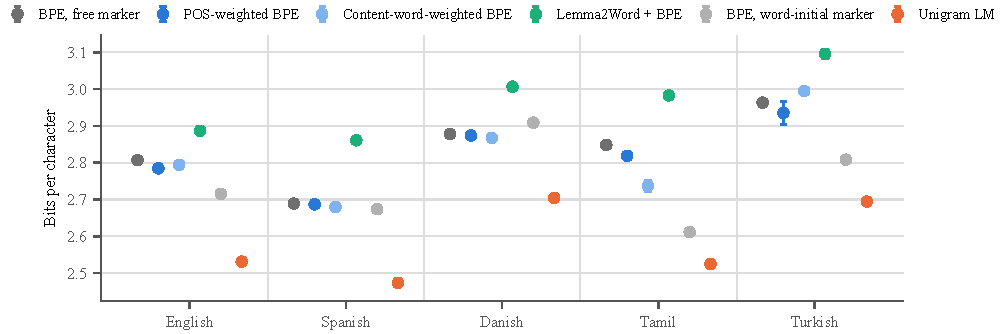
\includegraphics[width=\linewidth]{figures/fig_bpc.pdf}
\caption{Bits per character of a 7M-parameter language model trained for six passes over the same text with each tokenizer (lower is better). Points are means over the three tokenizer seeds and error bars span one standard deviation; the vertical axis starts at 2.4 bits so that the differences are visible.}
\label{fig:bpc}
\end{figure}

The ordering by bits per character is not the ordering by boundary F1.
The unigram model, second by F1, is first by a wide margin in every language, at \nBpcUniEnglish{} bits against \nBpcBpeEnglish{} for free-marker BPE in English and \nBpcUniTamil{} against \nBpcBpeTamil{} in Tamil.
Lemma2Word, first by F1 everywhere, is last by bits per character everywhere (\nBpcLtwEnglish{} in English).
Cutting words at the stem boundary before subword training removes frequent whole-word tokens from the vocabulary, and the extra tokens it produces are not predictable enough, for a model of this size, to pay for themselves.
The word-initial-marker BPE, last by F1 in four languages, is better than free-marker BPE by bits per character in four languages (\nBpcHfBpeEnglish{} against \nBpcBpeEnglish{} in English); the tokens that span word boundaries, which make the free-marker variant more compact, do not help prediction.
The POS weighting changes bits per character by less than 0.03 in every language, in the direction of a small improvement, with the largest seed-to-seed variation of the table in Turkish, and its two ablations again coincide with it.
The content-word weighting lowers bits per character in Tamil (\nBpcPosContentTamil{} against \nBpcBpeTamil), where it also raised boundary F1 most, and raises them in Turkish.

Because every model is trained for six passes over the same text, a tokenizer that produces more tokens also gives its model more optimizer steps, 8.6\% more for the unigram model than for free-marker BPE in English.
A control that trains the free-marker BPE model of seed 0 for 5.4 and 6.6 passes, 10\% fewer and 10\% more steps, moves its bits per character from \nBpcControlBase{} to \nBpcControlLow{} and \nBpcControlHigh{}, far less than the gaps between tokenizers, and Lemma2Word produces more tokens than free-marker BPE yet scores worse, so the step count does not explain the ordering.
What the probe shows is that morphological alignment and modeling quality do not move together at this scale, in agreement with \citet{bostrom2020bpe} on the unigram model and with the broader finding that intrinsic tokenizer measures predict downstream quality imperfectly~\cite{schmidt2024tokenization,ali2024tokenizer}.
